\documentclass[review]{elsarticle}

\usepackage{lineno,hyperref}
\usepackage{color}
\usepackage{url}
\usepackage{subfigure}
\usepackage{mathtools}
\modulolinenumbers[5]

\journal{Journal of \LaTeX\ Templates}

%%%%%%%%%%%%%%%%%%%%%%%
%% Elsevier bibliography styles
%%%%%%%%%%%%%%%%%%%%%%%
%% To change the style, put a % in front of the second line of the current style and
%% remove the % from the second line of the style you would like to use.
%%%%%%%%%%%%%%%%%%%%%%%

%% Numbered
%\bibliographystyle{model1-num-names}

%% Numbered without titles
%\bibliographystyle{model1a-num-names}

%% Harvard
%\bibliographystyle{model2-names.bst}\biboptions{authoryear}

%% Vancouver numbered
%\usepackage{numcompress}\bibliographystyle{model3-num-names}

%% Vancouver name/year
%\usepackage{numcompress}\bibliographystyle{model4-names}\biboptions{authoryear}

%% APA style
%\bibliographystyle{model5-names}\biboptions{authoryear}

%% AMA style
%\usepackage{numcompress}\bibliographystyle{model6-num-names}

%% `Elsevier LaTeX' style
\bibliographystyle{elsarticle-num}
%%%%%%%%%%%%%%%%%%%%%%%

\newcommand{\todo}[1]{{\color{red} [#1]}}
\newcommand{\fodo}[1]{\todo{\footnote{\todo{#1}}}}
\newcommand{\todots}{\todo{\ldots}}
\newcommand{\totalStudents}{227~}
\newcommand{\hypRange}{72\%~}

\begin{document}

\begin{frontmatter}

\title{30 Days After Introducing Programming:\\Will My Students Fail?}

%\title{A Strategy to Early Identify Potential Failing Students in Introductory Programming Courses}
%\tnotetext[mytitlenote]{Fully documented templates are available in the elsarticle package on \href{http://www.ctan.org/tex-archive/macros/latex/contrib/elsarticle}{CTAN}.}

%% Group authors per affiliation:
%\author{M\'{a}rcio Ribeiro}
%\address{Radarweg 29, Amsterdam}

%% or include affiliations in footnotes:
\author[ufal]{M\'{a}rcio Ribeiro}
\ead{marcio@ic.ufal.br}

\author[ufal]{Rodrigo Paes\corref{mycorrespondingauthor}}
\cortext[mycorrespondingauthor]{Corresponding author}
\ead{rodrigo@ic.ufal.br}

\author[ufcg]{Rohit Gheyi}
\ead{rohit@dsc.ufcg.edu.br}

\address[ufal]{Federal University of Alagoas, Macei\'{o}, Brazil}
\address[ufcg]{Federal University of Campina Grande, Campina Grande, Brazil}

\begin{abstract}
The high rate of failing students in introductory programming courses is a common problem. In this context, previous work revealed data and reasons regarding why students fail the courses. Despite these advances, there is a lack of an approach to identify, during the course, that a particular set of students will fail. By having this set, professors and mentors would have time to act and potentially avoid such failings. This way, this paper proposes a strategy to early identify failing students during introductory programming courses. We apply our strategy considering the first 30 days of the course. To evaluate our strategy, we conduct an empirical study regarding 7 courses (3.5 years in total). The study reveals that, from the group of students our strategy points as ``likely to fail,'' 72\% of the students indeed fail with 95\% standard confidence level. In addition, despite missing 28\%, this set seems still interesting, since at least 33\% of these students reach the final exam. Therefore, although they pass, we still consider they are good candidates to give special attention as well, which may avoid final exams and lead to better grades.

%In addition, when considering the 28\% remaining, at least 33\% of the students reach the final exam, which means that, although they pass, they are good candidates 
%The study reveals that our strategy successfully identifies 72\% of the failing students with 95\% standard confidence level.

\end{abstract}

\begin{keyword}
Programming courses, clustering
\MSC[2010] 00-01\sep  99-00
\end{keyword}

\end{frontmatter}

\linenumbers

%assistants ==> mentors
%identify ==> predict
% terminar related
% terminar comentarios de Rohit

\section{Introduction}

Introductory programming courses are often perceived by the students as problematic~\cite{yadin-inroads-acm-11}. This understanding seems to be based on the high dropout rates, which has been observed in universities around the world, such as at the United States~\cite{bennedsen-sigcse-failure-rates-2007}, Finland~\cite{why-dropout-icer06}, and ours in Brazil.

To predict the students likely to succeed or fail, previous studies provide aptitude tests regarding programming activities. These studies focus on identifying qualitatively the student skills and consider many different variables from big, complicated, and time-consuming surveys. Also, they might bring subjectiveness due to the interview process. To perform the predictions, they use high school data~\cite{butcher-predictor-high-school-1985}, diagnostic tasks~\cite{simon-predictors-ace2006}, mental models~\cite{camel-2006}, and even games~\cite{lorenzenC06-mastermind-predictor-sigcse2008}. Thus, although we can predict the potential failing students by using these studies, setting, executing, and replicating them is hard, time consuming and require extra effort from the professors. 

In this context, there is a lack of an automatic approach capable of predicting a set of students that will fail. This way, professors and mentors would be able to act and consequently help them. To achieve promising results, however, this approach must accomplish two main requirements. First, it must correctly predict as soon as possible, otherwise there will be not enough time to act and the student would drop out the course anyway. Also, due to the strong prerequisites of understanding previous classes to understand the current one in programming courses (e.g., to understand loops, students must understand conditional structures), the situation gets worse, even when acting just a bit late. Second, the approach must be automatic, requiring almost no effort from professors and mentors and allowing them to use it in every course they teach.

%When considering programming courses, the situation gets worse, even when acting just a bit late, due to the strong prerequisites of understanding previous classes to understand the current one (e.g., to understand loops, students must understand conditional structures). Second, the approach must require almost no effort from professors and mentors, otherwise they might not use it.


%Previous research introduce predictors to identify these students. However, they use aptitude tests and surveys to qualitatively identify the student skills and decide whether the student will succeed or fail~\cite{butcher-predictor-high-school-1985, simon-predictors-ace2006, camel-2006}. They also consider lots of variables, which makes the studies hard to replicate and to execute, being time consuming and increasing the professor effort.


%To reduce effort, the prediction must be automatic, requiring .

%However, identifying potential failing students during introductory programming courses is a non-trivial task~\cite{}, specially if we consider that this identification must be done as soon as possible, otherwise there will be no enough time to act and the student will drop out the course anyway. When considering programming courses, the situation gets worse even when acting just a bit late, due to the strong prerequisites of understanding previous classes to understand the current one (e.g., to understand loops, students must understand conditional structures).

%we often apply aptitude tests \textit{before} the enrolments. 

%~\cite{yadin-inroads-acm-11}. In particular, this problem has been seen in universities around the world, such as at the United States~\cite{bennedsen-sigcse-failure-rates-2007}, Finland~\cite{why-dropout-icer06}, and ours in Brazil. Due to such high failing rates, these courses are often perceived by the students as problematic~\cite{yadin-inroads-acm-11}. In this context, by analyzing the several reasons of why students fail~\cite{why-dropout-icer06}, such as lack of motivation, lack of time, and the chosen programming language, previous work report approaches to reduce these rates~\cite{yadin-inroads-acm-11, xxx}.

%These studies focus on data, reasons, and characteristics \textit{after} the student fail. Nevertheless, there is a lack of an approach capable of identifying that students are not comfortable still during the course. This way, professors and mentors would be able to act and consequently help them. However, identifying potential failing students during introductory programming courses is a non-trivial task~\cite{}, specially if we consider that this identification must be done as soon as possible, otherwise there will be no enough time to act and the student will drop out the course anyway. When considering programming courses, the situation gets worse even when acting just a bit late, due to the strong prerequisites of understanding previous classes to understand the current one (e.g., to understand loops, students must understand conditional structures).

To minimize this problem, in this article we propose an automatic strategy to early predict failing students in introductory programming courses. Our strategy consists of three simple steps. The first one is to make students use an online judge system. This kind of system executes an online submitted solution to a given problem against a set of predefined test cases to check whether the solution is correct or not. Then, we collect metrics of each student by using such a system. Finally, we execute a clustering algorithm~\cite{hartigan-clustering-algorithms-1975} to form groups so that we are able to separate the potential failing students from the other ones.

To evaluate our strategy, we conduct an empirical study regarding 7 introductory programming courses---3.5 years---with, in total, \totalStudents freshmen students (32 per course, on average). The courses focused on the C language and have been given by the same professor at the Federal University of Alagoas in Brazil. We apply our strategy considering the first 30 days of the programming course (25\% of a semester). The results suggest that our strategy can early predict the majority of the failing students within only 30 days. In particular, from the group of students our strategy points as ``likely to fail,'' 72\% of the students indeed fail with 95\% standard confidence level. Moreover, we observe that the 28\% our strategy misses is still important to take into account, since at least 33\% of these students have difficulties to pass and reach the final exam. So, although they pass, this set has good candidates that need special attention as well. Also, we conclude that the efficacy of our strategy can strongly depend on the number of students in the course. Because the strategy is automatic, the effort to predict the potential failing students in a course with hundreds~\cite{bennedsen-sigcse-failure-rates-2007} can significantly reduce. In case the course has few students (e.g., 10 students), we report that our strategy adds little, since the own professor can identify the failing candidates.

%In case professors and mentors help these students, they may avoid final exams and achieve better grades at the end of the course.

In summary, this article provides the following contributions:

\begin{itemize}

	\item A strategy to early predict automatically the potential failing students in introductory programming courses;
	
	\item An empirical study assessing the potential of our strategy. We evaluate our strategy by using \totalStudents students from 7 courses during 3.5 years, demonstrating significant potential.

\end{itemize}

We organize the remainder of this article as follows. Section~\ref{sec:problem} discusses in detail the problem we address in this work. Then, Section~\ref{sec:strategy} introduces our strategy and details the three steps we consider. Section~\ref{sec:evaluation} presents the evaluation we perform whereas Section~\ref{sec:results} discusses the results and findings. We then discuss the related work in Section~\ref{sec:related}. Last but not least, we present the concluding remarks in Section~\ref{sec:conclusion}.

\section{Problem}

\label{sec:problem}

Professors often are not aware of what actually hinders particular students during the learning process. Another difficulty consists of pointing out the exactly students that need help, specially when considering courses with hundreds of enrolled students~\cite{bennedsen-sigcse-failure-rates-2007}. With no support, students might have no enthusiasm regarding the classes and get frustrated and disappointed, leading them to fail the course.

In this context, there is no straightforward way to predict the potential failing students during introductory programming courses. When professors and mentors do not early identify such students, they may act too late---or even may not act, since there is no available time anymore---and the students drop out the course anyway. In case they act just a bit late, they still face the hard task of recovering such students, which happens to be even harder in programming courses. Here, to understand the next class there is a strong prerequisite of understanding the previous ones (e.g., to understand loops, students must understand conditional structures). 

So, not identifying failing students early is a critical problem, specially when we consider that programming is one of the first courses that students face in their computer science university program. If these courses have as high failure rates as claimed, they could be one of the factors influencing the declining number of students taking a degree in computer science \cite{bennedsen-sigcse-failure-rates-2007}.

Previous research introduce predictors to identify these students. However, they use aptitude tests and surveys to qualitatively identify the student skills and decide whether the student will succeed or fail~\cite{butcher-predictor-high-school-1985, simon-predictors-ace2006, camel-2006}, which might bring subjectiveness due to the interviews. They also consider lots of variables, which makes the studies hard to set, execute, and replicate, being time consuming and increasing the professor effort. So, it is difficult to gather and analyze this information at the beginning of the semester~\cite{harris-assembly-jcsc2014} to determine the students candidates to fail. Although automatic approaches have been proposed~\cite{}, they predict the failing students either too late or with moderate precision.

To sum up, we rise three challenges we intend to address: to predict the failing students (i) as soon as possible; (ii) with high precision; and (iii) automatically. To do so, we present in the next section a strategy to early predict the potential failing students in introductory programming courses automatically. Our strategy consists of three simple steps and it is automatic and objective (relying on metrics), reducing effort and allowing professors to use it in their courses.

%Due to the high number of students, professors and mentors might face difficulties to identify the potential failing students during the courses they teach. In this context, professors often are not aware of what actually hinders particular students during the learning process. With no additional help, students have no enthusiasm regarding the classes and get frustrated and disappointed, leading them to fail the course.


%specially when they see their friends excited about the course. This situation causes shame and timidity, which may lead them to not ask questions or not participate in class. When considering introductory programming courses, this frustration may lead students to fail the course.



%Why the problem is relevant, important?
%In this context, there is no easy way to \textit{early} identify potential failing students during introductory programming courses. When professors and mentors do not early identify students that tend to fail the programming course, they may act too late---or even may not act, since there is no available time anymore---and the students drop out the course anyway. In case they act a bit late, they still face the hard task of recovering such students, which happens to be even harder in programming courses. In this context, to understand the next class there is a strong prerequisite of understanding the previous ones (e.g., to understand loops, students must understand conditional structures).

%This way, not identifying failing students early is a critical problem, specially when we consider that programming is one of the first courses that students face in their computer science university program. If these courses have as high failure rates as claimed, they could be one of the factors influencing the declining number of students taking a degree in computer science \cite{bennedsen-sigcse-failure-rates-2007}.

%Notice that the problem of identifying failing students is even more critical when considering courses with high number of enrolled students. \todots



%\todo{Relevar mais o problema do dropout rate. Fico com medo de fugir um pouco do escopo. O problema e identificar cedo ou o high dropout rate??? Ou a relev�ncia do early esta no sentido que, ao nao identificar, temos high rates?}

%\todo{Citar as linguagens desses papers com high dropout. Pegar dados de outros artigos. Dos nossos cursos tamb�m.}

%To minimize the lack of an early identification of potential failing students that would enable professors and mentors to act faster in order to avoid such failings, we next present a strategy that consists of three simple steps: the use of a online judge system, metrics collection, and execution of a well-known clustering algorithm~\cite{hartigan-clustering-algorithms-1975}.


%Due to the high number of students, professors and mentors might face difficulties to identify the potential failing students during the courses they teach. In this context, professors often are not aware of what actually hinders particular students during the learning process. With no additional help, students have no enthusiasm regarding the classes and get frustrated and disappointed, leading them to fail the course.


%specially when they see their friends excited about the course. This situation causes shame and timidity, which may lead them to not ask questions or not participate in class. When considering introductory programming courses, this frustration may lead students to fail the course.

\section{Early detection of potential dropout students}

\label{sec:strategy}

This way, the problem we address in this paper consists of a strategy to \textit{early} identify potential failing students. Notice that identifying early is very important in the sense that professors still have enough time to act and avoid students to fail the course. This way, we focus exclusively on early identifying these students. Providing or reporting a technique useful to reduce the failure rate is outside the scope of this paper. Nevertheless, notice that when identifying them we may study the data and afterwards provide a technique to do so. Actually, based on the results of this paper, we intend to propose a technique to reduce the failure rate as future work.

Next, we detail our strategy to identify these students.

\subsection{Online judge system}
% This section should answer: Why is this kind of system important to identify potential falling students?
% Answer: We need metrics. In order to discover how students are performing, it is necessary a close monitoring of students behaviour
% Talk about Huxley, only enough to explain the metrics: submissions and submission_status (Correct ...)
In order to discover how students are performing, it is important to define a strategy to close monitoring students’ behavior. This strategy should include a way to extract metrics from students. Online learning tools may be a source for these metrics. In the context of programming, a very popular category of systems is the online judges. These systems present students to a set or programming problems. The students solve the problem using a programming language and then submits their solutions. The online judge runs the student’s solution against a set of test cases and in the case the solution passes over all the tests it will be evaluated as correct, otherwise, it will be evaluated according to the type of error, such as wrong answer, compilation error, runtime error, etc.

% Why the Huxley and not others?
% answer: Metrics and performance improvement (not in scope)
In our strategy, we choose to use an online judge named \emph{The Huxley} \cite{paes2013ferramenta} to collect metrics from our students. In this system, the judge provides one of the following outputs for a submission: correct, wrong answer, time limit exceeded, compilation error, runtime error, presentation error and empty answer. We will use these outputs as the main source of metrics. This particular online judge system was chosen because it has some features that we believe will be useful to improve the overall performance of students as a future direction of this research. More specifically, the tool will support us to deal with the following problems:
\begin{itemize}
  \item Students only learn how to program by programming~\cite{jenkins-ltsn02}. The Huxley provides a database composed of more than 300 problems. It allows students to submit their solutions to any of these problems and they are encouraged to try once mistakes are not penalized.
  \item Sometimes a student who misses a basic concept and then cannot follow the next lecture. She believes that there is no going back; the course is behaving is a speed that she thinks she will be not able to follow. Such a student will quickly come to the view that ``they just cannot do programming'', and will attribute this to the perceived difficulty of the subject. In other words, students learn at different speeds. As the tools is available online on the Internet, each student can find its own rhythm on an extra class schedule.
  \item Students need rapid feedback. Many professors are overwhelmed with their daily activities. Then they have no time to give feedback on every student code. On the other side, students need this feedback to continue their learning process in the right path. The Huxley provides a feedback right after the student submits her code. The feedback indicates whether user produces the right answer and gives tips in the case user otherwise.
  \item There always be great students and bad students. The great ones should be presented to challenges that make them even greater and the bad ones should be presented to a different set of problems that allow them to become better. Each programming problem of the Huxley is classified according to this level of difficulty and the programming topics it covers. This allows each student to choose the next problem in accordance with this level of expertise.
\end{itemize}

\subsection{Metrics}

\label{sec:metrics}

We use two metrics in our strategy. We explain them in what follows:

\begin{itemize}

	\item \textbf{Number of submissions:} this metric represents the number of submissions a student do during the course. As explained, Huxley provides more than 300 programming exercises. To solve a particular problem, a student needs to submit at least one solution.

	\item \textbf{Number of correct submissions:} if a student solves one problem, we increase this metric by one.

\end{itemize}

Depending on the level of difficulty of a problem, students may submit several times to solve it. However, notice that this is not necessarily a bad thing regarding the learning process. For example, submitting many times means that students are somehow practicing and studying continuously. Thus, although she is not hitting a right solution, she is trying hard and will eventually hit one. Nevertheless, we need to carefully analyze \todots

\todo{Por que essas metricas sao boas? Por que escolhemos elas? O texto acima ajuda a explicar isso? Essas metricas nao sao obvias?}

\subsection{Clustering algorithm}

To identify potential failing students, we use the well-known clustering algorithm k-means~\cite{}. As input, we set the algorithm to compute three groups. To compute the groups, the algorithm takes into account the metrics we present in Section~\ref{sec:metrics}.

We choose three groups because ???

\todo{Por que escolhemos clustering? Por que o k-means?}

\todo{Por que 3 grupos? O do meio seria impossível prever algo. Mas isso nao e obvio?}

\subsection{Summary}

Figure~\ref{fig:strategy} combines all steps of our strategy. As the classes are happening, students are encouraged to solve exercises using the problems of Huxley. Although solving exercises is not mandatory, there some particular activities where the professor forces students to use Huxley. Next, we collect the metrics we detail in Section~\ref{sec:metrics}. To identify potential failing students \textit{early}, we collect the metrics for the first 30 days of the introductory programming courses. Then, we execute the k-means clustering algorithm.

%Then, we execute a R script we implemented to execute the clustering algorithm. As can be seen, there are three groups, represented by circles, squares, and stars. \todo{falar dos 30 dias}

\begin{figure}[htb]
\centering
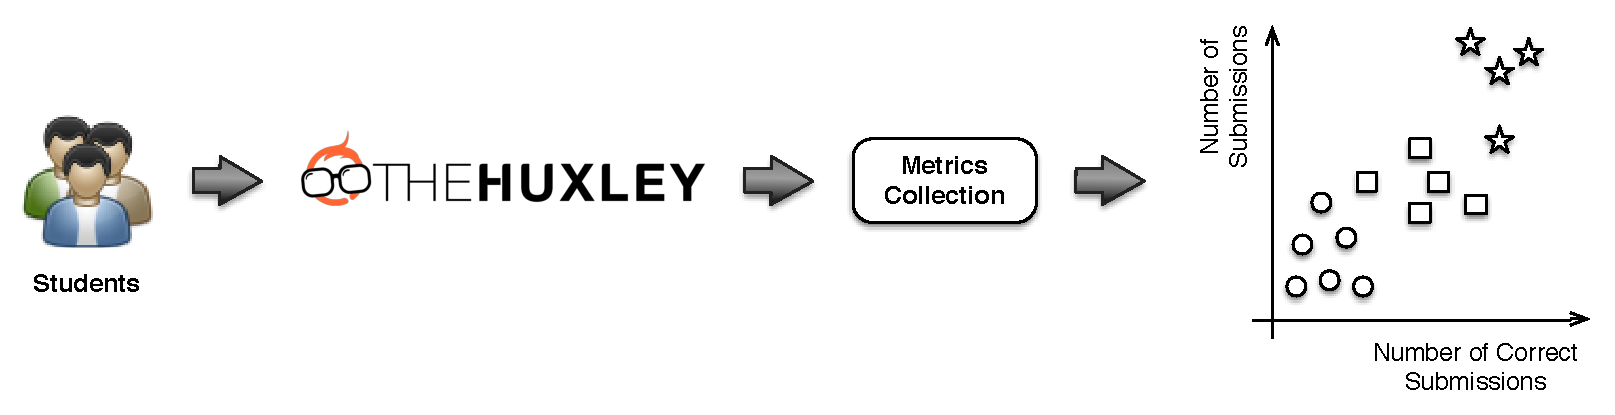
\includegraphics[width=1.0\textwidth,natwidth=610,natheight=642]{images/Strategy.pdf}
\caption{Summary of our strategy to identify potential failing students.}
\label{fig:strategy}
\end{figure}


\section{Evaluation}

\label{sec:evaluation}

To evaluate our strategy, in this section we present the empirical study we conduct. The objective of this study is to evaluate to what extent our strategy is capable of identifying potential failing students in only 30 days. To explain our evaluation design, we first present the participants and material in Section~\ref{sec:participants}. Then, we detail the procedure we use during the evaluation in Section~\ref{sec:procedure}.

%Before explaining our study, we first introduce the terminology we use throughout this paper. In particular, we define in what follows four categories: abort, skip, fail, and pass.
%
%\begin{itemize}
%
%	\item \textbf{Abort:} students that aborted the course before the final exam;
%	\item \textbf{Skip:} students allowed to do the final exam but did not show up;
%	\item \textbf{Fail:} students who failed the course;
%	\item \textbf{Pass:} students who successfully passed the course.
%
%\end{itemize}

%Now, we present the objetives and hypothesis (Section~\ref{sec:hypotheses}) of our study, then the participants and material (Section~\ref{sec:participants}) we use, and finally we detail the procedure (Section~\ref{sec:procedure}) we use during the evaluation.

%\subsection{Objective and Hypothesis}

%\label{sec:hypotheses}

%The objective of this study is to evaluate to what extent our strategy is capable of identifying potential failing students. This way, based on this objective, our hypothesis is the following: In the first 30 days, students with lower number of submissions and correct submissions tend to fail the course.

\subsection{Participants and Material}

\label{sec:participants}

The participants of our study are students of introductory programming courses at the Federal University of Alagoas, Brazil. We ministered these courses during 3.5 years and collected the metrics we detail in Section~\ref{sec:metrics} of each student by using Huxley. The professor encouraged all students to use Huxley to practice by solving the available problems. The use of Huxley was mandatory only during formal exams. Table~\ref{tab:participants} distribute the number of participants per semester.

\begin{table}[h]
\centering
\begin{tabular}{|c|c|}
\hline
\textbf{Course} & \textbf{Number of enrolled students}\\ \hline
2010.02 & 32\\ \hline
2011.01 & 38\\ \hline
2011.02 & 35\\ \hline
2012.01 & 34\\ \hline
2012.02 & 29\\ \hline
2013.01 & 28\\ \hline
2013.02 & 31\\ \hline
\textbf{TOTAL:} & \totalStudents\\ \hline
\end{tabular}
\caption{Participants per course.}
\label{tab:participants}
\end{table}

The material of this study consists of almost 300 programming exercises in Huxley. They were available for all students of all courses we use in this paper.

\todo{Descrever: quantas submissoes; linguagem C; mesmo professor; quantos problemas? focar somente nos 30 dias? Teve prova nos 30 dias?}

\todo{Colocar um exemplo de problema. Print screen da tela do huxley? Traduzir para ingles. Nivel de dificuldade? Problemas simples? Colocar uma lista de uns 30 problemas?}

\todo{O que foi feito nos cursos? Aulas expositivas? Listas de exercicios? Importante para qualquer outro professor replicar.}

\subsection{Procedure}

\label{sec:procedure}

Figure~\ref{fig:procedure} illustrates how we perform our evaluation. The result of executing our strategy consists of groups of students according to the clustering algorithm. Now, according to the groups, we have the potential failing students (see the left-hand side in Figure~\ref{fig:procedure}). These students are the ones that have a small number of submissions and correct submissions (represented by circles). Notice we also have students that are potential candidates to successfully pass (represented by stars): due to the high number of submissions to Huxley after 30 days, they seem to be practicing programming really hard. We represent the inconclusive group by squares.

\begin{figure}[htb]
\centering
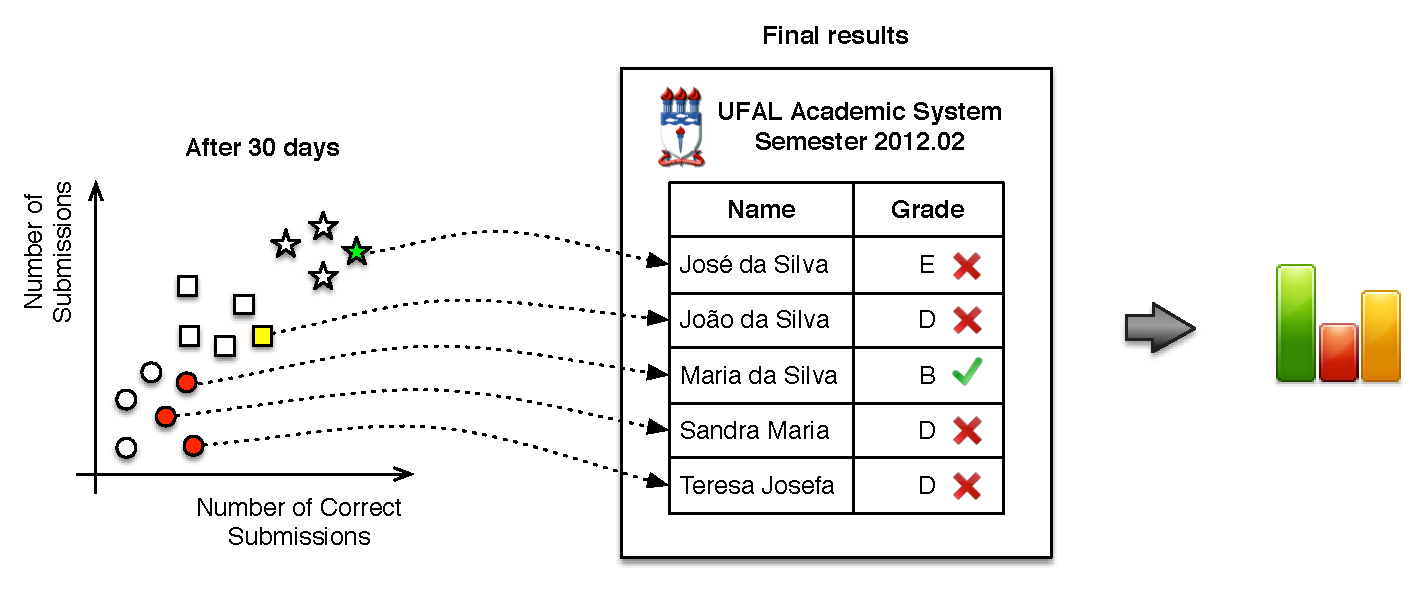
\includegraphics[width=1.0\textwidth,natwidth=950,natheight=394]{images/Procedure.pdf}
\caption{Checking the strategy results against the actual grades.}
\label{fig:procedure}
\end{figure}

After applying the strategy, we now need to check whether it correctly predicts the failing students after 30 days. To do so, we use the academic system of the Federal University of Alagoas to look for grades and check whether the students failed or not. For example, for the detached circles, the strategy successfully identified that, after 30 days, two students would not pass and they indeed did not. Notice, however, that we may face false positives. Despite indicating the student \textit{Maria da Silva}\footnote{All names we consider in this paper are fictitious.} as a failing one after 30 days, such a student seemed to improve herself during the semester and she has been approved. In addition, we may also have false negatives. For instance, our strategy does not point the students \textit{Jos\'{e} da Silva} and \textit{Jo\~{a}o da Silva} as failing ones. Although \textit{Jos\'{e} da Silva} seems to be one of the best students after 30 days, he failed the course. The several reasons why this happened is out of the scope of this paper.

To better structure and analyze our results and, at the same time, take false positives and false negatives into account, we consider the following two metrics: precision and recall. Precision is the fraction of retrieved students that are relevant, i.e., the students pointed by the strategy that indeed failed the course. We have a perfect precision, 1.0, when every student retrieved by the strategy is relevant (i.e., a failing student), which means we have no false positives. Precision focuses on \textit{quality} and \textit{accuracy}. However, the precision says nothing about whether \textit{all} relevant students were indeed retrieved.

\vspace{0.1cm}
$$
Precision = \frac{| \{relevant\_students\} \cap \{retrieved\_students\} |}{| \{retrieved\_students\} |}
$$
\vspace{0.1cm}

Recall, in its turn, is the fraction of relevant students that are retrieved, i.e., it is the probability of retrieving a failing student. A perfect recall, 1.0, means that we retrieve all failing students, which means we have no false negatives. In this context, recall focuses on \textit{completeness} and \textit{quantity}. Notice that recall says nothing about how many irrelevant students (students that will pass) the strategy retrieved.

\vspace{0.1cm}
$$
Recall = \frac{| \{relevant\_students\} \cap \{retrieved\_students\} |}{| \{relevant\_students\} |}
$$
\vspace{0.1cm}

To better explain these metrics, consider the detached students in Figure~\ref{fig:procedure} as our set (three circles, one square, and one star). The relevant set is \textit{\{Jos\'{e}, Jo\~{a}o, Sandra, Teresa\}}, whereas the retrieved set is \textit{\{Maria, Sandra, Teresa\}}. The intersection set is \textit{\{Sandra, Teresa\}}. This way, we have

\vspace{0.2cm}
\noindent
\scriptsize
\begin{minipage}{.5\linewidth}
\centering
$$
Precision = \frac{|\{Sandra, Teresa\}|}{|\{Maria, Sandra, Teresa\}|} = 67\%;
$$
\end{minipage}
\begin{minipage}{.5\linewidth}
$$
Recall = \frac{|\{Sandra, Teresa\}|}{|\{\textit{\text{Jos\'{e}}}, \textit{\text{Jo\~{a}o}}, Sandra, Teresa\}|} = 50\%.
$$
\end{minipage}
\normalsize
\vspace{0.2cm}

Our strategy pointed two out of three students as failed ones and they indeed failed. Therefore, we have 67\% of accuracy when identifying potential failing students, raising one false positive. On the other hand, only two out of four students have been pointed as failed ones. This means that the strategy was not able to identify all failing students, raising two false negatives.

Last but not least, after confronting the strategy results with the academic system and summarizing precision and recall, we apply a statistical test to check for significance. Here, we rely on the proportion statistical test based on the Bernoulli distribution~\cite{} so that we have a binary distribution: fail or pass. In this paper, we follow the convention of considering a factor as being significant to the response variable when \textit{p-value} $< 0.05$~\cite{}.

\section{Results and Discussion}

In this section, we describe the results and test our hypotheses before discussing their implications. All data, materials, and R scripts are available at \url{http://www.ic.ufal.br/}.

\subsection{Results}

In our evaluation, we use data of 7 courses (3.5 years) totalling \totalStudents students. We apply our strategy by setting k-means to compute two and three groups. We now proceed separately, reporting the results considering both cases.

\subsubsection{Two groups}

When considering two groups, we set the strategy to consider all students in two categories: fail or pass. Figure~\ref{fig:2-groups} illustrates the results for all courses. Notice that Figure~\ref{fig:2-2011-01} contains an outlier. In this particular case, the strategy pointed that all students but one would fail the course. Clearly this result is a consequence of such outlier. This way, the presence of one outlier might represent a problem when considering two groups.

\begin{figure*}[ht]
     \begin{center}
         \subfigure[2010.02] {
             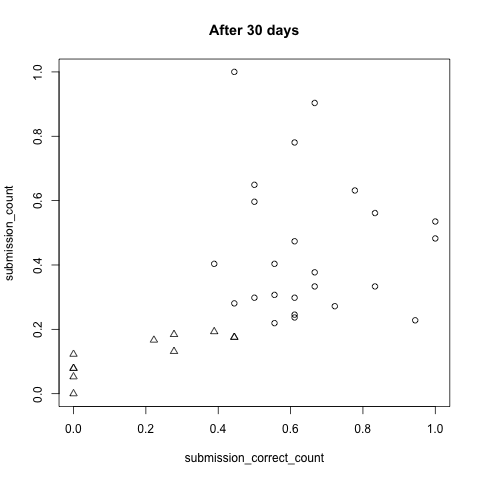
\includegraphics[scale=0.21,natwidth=480,natheight=480]{images/2-2010-02.png}
             \label{fig:2-2010-02}
         }
         \subfigure[2011.01] {
             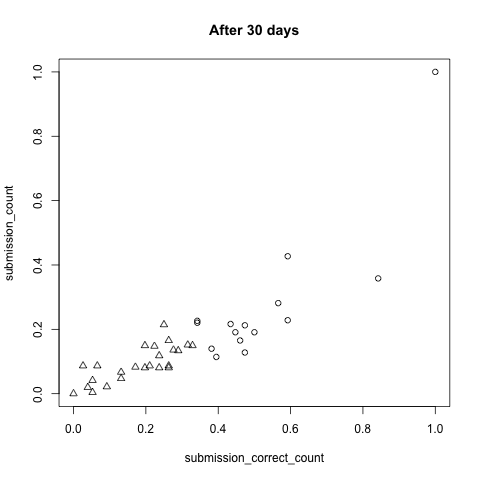
\includegraphics[scale=0.21,natwidth=480,natheight=480]{images/2-2011-01.png}
             \label{fig:2-2011-01}
         }
         \subfigure[2011.02] {
             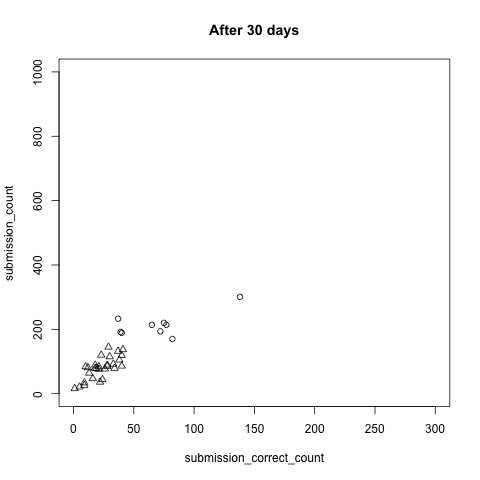
\includegraphics[scale=0.21,natwidth=480,natheight=480]{images/2-2011-02.png}
             \label{fig:2-2011-02}
         }
         \subfigure[2012.01] {
             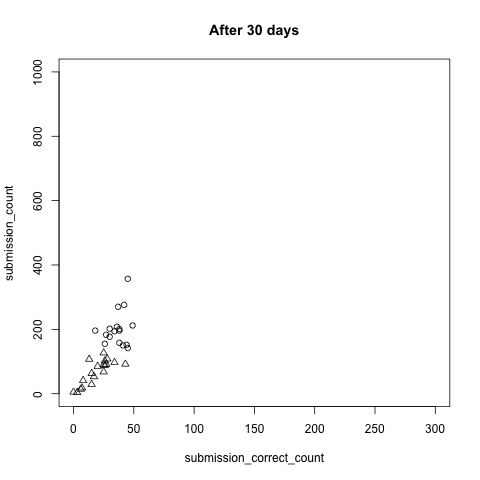
\includegraphics[scale=0.21,natwidth=480,natheight=480]{images/2-2012-01.png}
             \label{fig:2-2012-01}
         }
         \subfigure[2012.02] {
             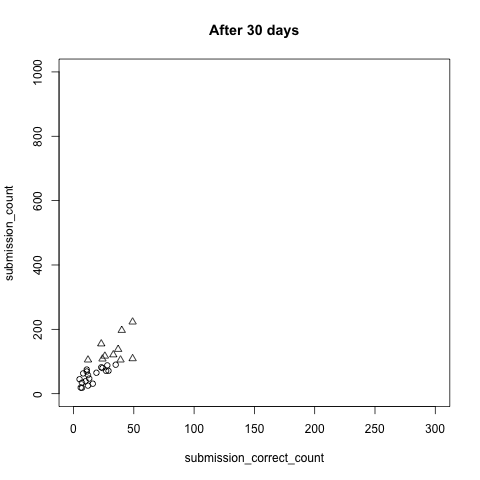
\includegraphics[scale=0.21,natwidth=480,natheight=480]{images/2-2012-02.png}
             \label{fig:2-2012-02}
         }
         \subfigure[2013.01] {
             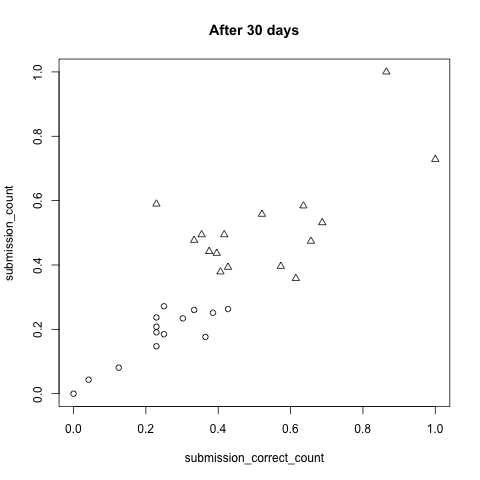
\includegraphics[scale=0.21,natwidth=480,natheight=480]{images/2-2013-01.png}
             \label{fig:2-2013-01}
         }
         \subfigure[2013.02] {
             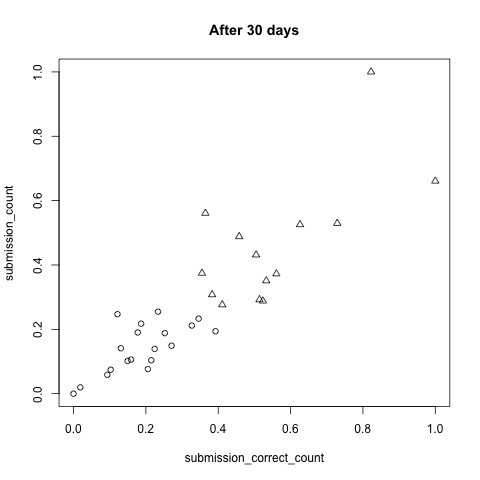
\includegraphics[scale=0.21,natwidth=480,natheight=480]{images/2-2013-02.png}
             \label{fig:2-2013-02}
         }
     \end{center}
     \caption{Strategy applied with two groups.}
	 \label{fig:2-groups}
\end{figure*}

To better analyze our results, we remove this outlier and execute our strategy again. By using two groups and properly removing the outlier, we achieve the following results for precision and recall:

\vspace{0.2cm}
\noindent
\begin{minipage}{.5\linewidth}
\centering
$$
Precision = \frac{92}{145} = 63\%;
$$
\end{minipage}
\begin{minipage}{.5\linewidth}
$$
Recall = \frac{92}{115} = 80\%.
$$
\end{minipage}
\vspace{0.2cm}

Here we observe a high recall, i.e., 80\%. This means we only miss 20\% of the failing students. We have few false negatives, but this result says nothing about how many false positives (irrelevant students) we retrieved. However, notice that this result (80\%) represents our particular sample. We now need to find the population proportion, enabling us to generalize our findings. To do so, we need to check for statistical significance by executing the proportion hypothesis test. In this context, the test reveals that the population recall is 73\% with a confidence level of 95\% (\textit{p-value} $= 0.045$). Regarding precision, our results show a sample precision of 63\%. To generalize, we again execute the test and find that the population precision would be 56\% (\textit{p-value} $= 0.035$).

\subsubsection{Three groups}

Analogously, we set our strategy to consider three groups. Here, besides the failing and passing groups, there is one extra group where the strategy cannot conclude anything about it. Figure~\ref{fig:3-groups} shows the results for three groups. Differently from two groups, here one outlier does not completely compromise the strategy.

\begin{figure*}[ht]
     \begin{center}
         \subfigure[2010.02] {
             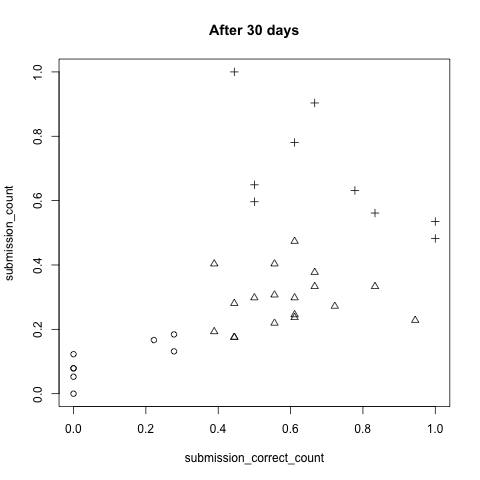
\includegraphics[scale=0.21,natwidth=480,natheight=480]{images/3-2010-02.png}
             \label{fig:3-2010-02}
         }
         \subfigure[2011.01] {
             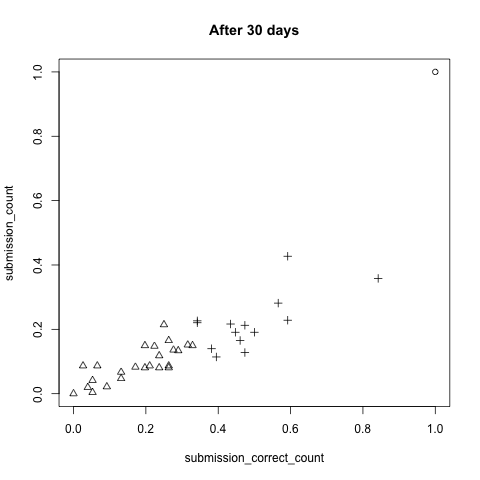
\includegraphics[scale=0.21,natwidth=480,natheight=480]{images/3-2011-01.png}
             \label{fig:3-2011-01}
         }\\
         \subfigure[2011.02] {
             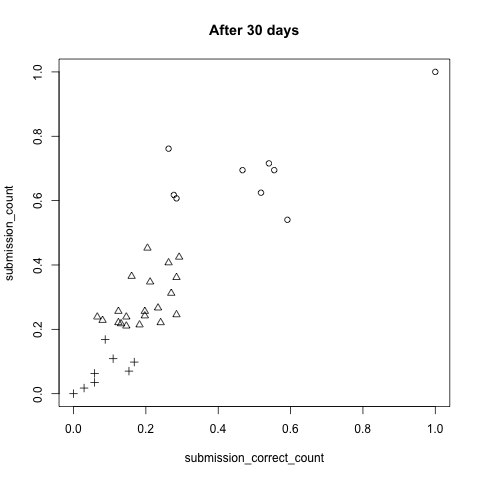
\includegraphics[scale=0.21,natwidth=480,natheight=480]{images/3-2011-02.png}
             \label{fig:3-2011-02}
         }
         \subfigure[2012.01] {
             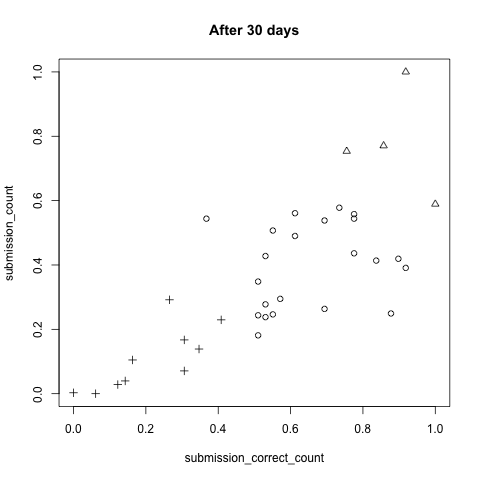
\includegraphics[scale=0.21,natwidth=480,natheight=480]{images/3-2012-01.png}
             \label{fig:3-2012-01}
         }\\
         \subfigure[2012.02] {
             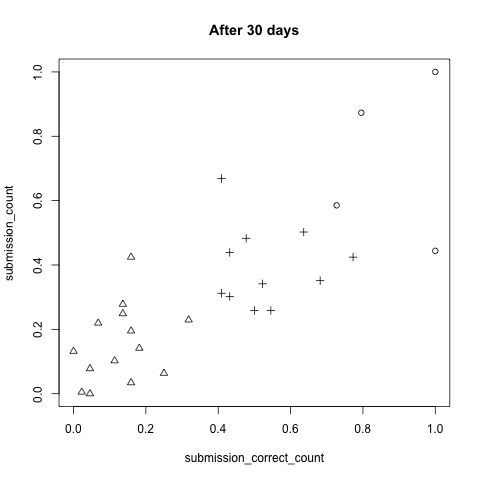
\includegraphics[scale=0.21,natwidth=480,natheight=480]{images/3-2012-02.png}
             \label{fig:3-2012-02}
         }
         \subfigure[2013.01] {
             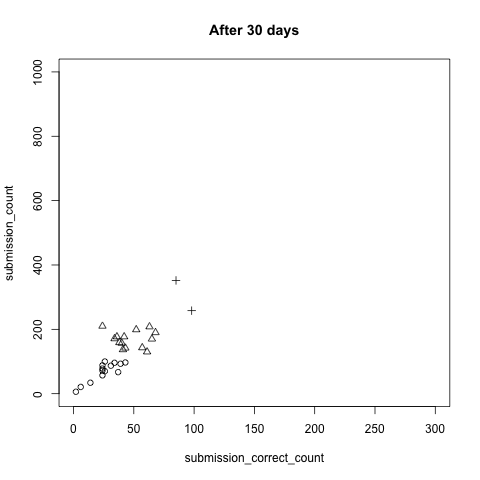
\includegraphics[scale=0.21,natwidth=480,natheight=480]{images/3-2013-01.png}
             \label{fig:3-2013-01}
         }\\
         \subfigure[2013.02] {
             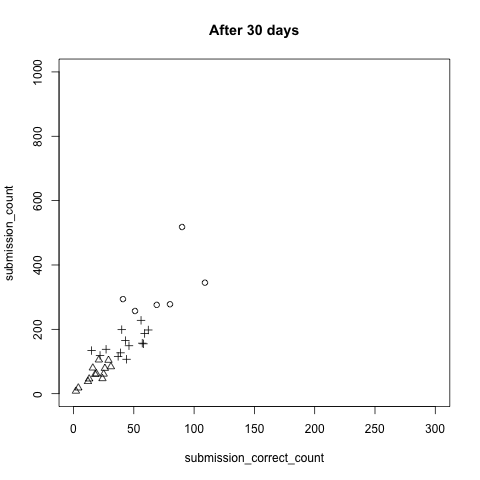
\includegraphics[scale=0.21,natwidth=480,natheight=480]{images/3-2013-02.png}
             \label{fig:3-2013-02}
         }
     \end{center}
     \caption{Strategy applied with three groups.}
	 \label{fig:3-groups}
\end{figure*}

We present the precision and recall for three groups in what follows:

\vspace{0.2cm}
\noindent
\begin{minipage}{.5\linewidth}
\centering
$$
Precision = \frac{73}{91} = 80\%;
$$
\end{minipage}
\begin{minipage}{.5\linewidth}
$$
Recall = \frac{73}{115} = 63\%.
$$
\end{minipage}
\vspace{0.2cm}

Now the strategy returns a precision of 80\% for the sample proportion. To generalize our results, we again execute the proportion hypothesis test. Regarding the population, our results reveal that the precision is 72\% with a confidence level of 95\%. In other words, from the set we retrieve,  we can identify with statistical significance (\textit{p-value} $= 0.04$) 72\% of the students that indeed will fail the course after 30 days. We repeat this process for recall and find 63\% for the sample and 55\% for the population, \textit{p-value} $= 0.033$.

Notice that with three groups the results of precision and recall are inverted when compared to two groups. Our strategy uses k-means, which takes into account two metrics---number of submissions and number of correct submissions---and the number of groups. Both executions are totally independent and the algorithm is not aware of precision, recall, and the academic system. Therefore, we take these results as a coincidence.

\subsection{Discussion}

In this section we discuss the results. We first discuss the number of groups we should set when using our strategy and then we discuss our achievements regarding final exams.

\subsubsection{Two or Three Groups?}

When applying our strategy considering two groups, the results indicate a higher recall when compared to three groups. This means that the strategy can identify the majority of the failing students (raising only few false negatives). Although this is an interesting result, the strategy with two groups yields many false positives. In fact, the precision is lower when compared to three groups, i.e., the set we retrieve contains many students that pass. In this situation, professors and assistants might waste effort trying to recover students that actually do not need recovering. On the other hand, with three groups we have a higher precision, which means professors should give special attention to the students the strategy retrieves, since 72\% of them tend to fail. Nevertheless, since the recall is lower than with two groups, we have more failing students not retrieved by the strategy for three groups.

%we may have there are many failing students not retrieved by the strategy.

In this context, setting the number of groups to execute our strategy seems to depend on the professors priorities and resources. In case the professor has available time and additional assistants to help her, she can probably use two groups, which consists of a more complete retrieved set (the recall is higher for two groups), even though it contains many false positives. However, notice that applying the strategy with two groups is more likely to outliers problems, such the one we depict in Figure~\ref{fig:2-2011-01}.

On the other hand, if the professor wants to avoid false positives because of no available time or few assistants to help, she might prefer to use three groups, despite being aware of potential failing students not retrieved by the strategy (many false negatives, lower recall than with two groups). 

%better precision in exchange for 

\subsubsection{Final Exams}

Even though the strategy pointed students as potential failing ones in the first 30 days, some of them passed, raising false positives. Table~\ref{tab:final-exams} illustrates the precision for two and three groups as well as the false positives. For two and three groups, the precision is 56\% and 72\%, respectively. This way, we have 44\% and 28\% of false positives. As mentioned, the number of false positives is greater when considering two groups.

\begin{table}[h]
\centering
\begin{tabular}{|c|c|c|c|}
\hline
\textbf{Groups} & \textbf{Precision} & \textbf{False Positives} & \textbf{Final Exam}\\ \hline
2 & 56\% & 44\% (53 students) & 35\% (19 out of 53 students)\\ \hline
3 & 72\% & 28\% (18 students) & 33\% (06 out of 18 students)\\ \hline
\end{tabular}
\caption{False positives (students pointed as potential failing ones but passed) that performed the final exam.}
\label{tab:final-exams}
\end{table}

To better understand these false positives, we now analyze their grades at the academic system. In our study, we find that some of these students did not pass in the first place. In fact, they needed to perform the final exam to pass. At the university we focus on this paper, the final exam represents a second chance and is only available to students with not enough grades to pass.

This result is important in the sense that, although the strategy might raise false positives, it seems worth to follow these students as well. We find that at least 33\% of them need help (regardless of the number of groups, two or three), otherwise they reach the final exams. This way, professors and assistants can also give special attention to these students, which may improve their learning process, avoid final exams, and lead to better grades.

\subsubsection{Back to our objective}

As mentioned, the objective of our study is ``to evaluate to what extent our strategy is capable of identifying potential failing students in only 30 days.'' Given the results we achieve, we believe our strategy is indeed capable of identifying the failing students early. In particular, from the group of students our strategy points as ``likely to fail,'' 72\% of the students indeed fail with 95\% standard confidence level by using three groups. 

%Also, we notice that the 28\% remaining contains at least 33\% of students that somehow need help, since they reach the final exam.

\subsubsection{Dropout rate}

\todo{Discuss how the strategy can minimize the dropout rate. }

\subsubsection{Number of students}

The efficacy of our strategy can strongly depend on the number of enrolled students in the course. In this context, if the number of students is small (e.g., 10 students), the own professor can identify---also early---the students that need help. This scenario is even more promising when the professor counts on assistants to help. Therefore, in this situation, our strategy adds little and professors might not notice benefits of using it.

On the other hand, despite having courses throughout Brazil with few students, it is common to find courses with 30, 40, 50, or even 60 enrolled students. In USA, this number can be even larger at some universities. In this scenario, our strategy can better support professors and their assistants. \todots

\todo{It seems like the small classes (less than 30 students) do better than the larger ones---the average pass rate in the small classes is 82\% whereas large classes only have an average pass rate of 69\%~\cite{bulletin2007}.}

\todo{The size of the courses also varies a lot, from 8 students to 645. The mean course size is 116, but 23\% of the courses have less than 30 students~\cite{bulletin2007}.}

\todo{Citar na introducao que a estrategia funciona melhor para esses casos de turmas grandes.}

\subsubsection{Mini testes}

\todo{Posso aplicar muitos mini testes. Mas o esforco vai ser grande. Criar as questoes e corrigir. O uso do online judge ajuda.}

\todo{Bronca: Estrategia versus Tabela no huxley de scores nos exercicios. Como defender a estrategia? Por que o huxley sozinho nao e suficiente?}

\todo{Outra bronca: Fiz uma prova nos 30 dias, quem tirou nota ruim, vai perder. Qual a diferenca disso pra estrategia?

\begin{itemize}

	\item So uma prova, nao haveria muito feedback. Dia ruim?
	\item Varios minitestes, ha uma avalia��o constante; a quantidade de dados e feedback e muito maior!

\end{itemize}

}

\subsubsection{O que a estrategia oferece? Por que devo usa-la? Por que o que existe nao e suficiente?}

\begin{itemize}

	\item Automatico! Diminui o esforco para identificar.
	\item Boa precisao.
	\item 

\end{itemize}

\subsection{Threats to validity}

In this section we present the threats to validity of our study. Although our sample is reasonably big (227 students), our study has homogeneities that might pose threats. For example, the same professor for all the 7 courses and the same language used (C language) threats external validity. In this way, it is difficult to extrapolate the results to other contexts. Nevertheless, our strategy uses metrics to identify potential failing students. In this context, we argue that the metrics we use (submissions and correct submissions) do not necessarily depend on factors such as the professors and even less on the adopted languages. However, our claim is not enough and we need further studies to better generalize our conclusions.

The use of Huxley threats internal validity. Students must know how to use the system to submit their solutions. If the students somehow do not get used to the system, they might feel frustrated, hindering their learning and, consequently, biasing our results. We minimize this threat by introducing Huxley in the very first classes as well as by using assistants to help the students on how to use Huxley.

\section{Related Work}

\label{sec:related}

Reducing the failure rate in programming courses has been achieved in previous work~\cite{}. The authors performed a study during four semesters. They identified three main factors to reduce the failure rate: (i) using Python as the first introductory programming language, which, according to the authors, may lead the students to better focus on algorithms and problem solving, instead of spending time with advanced concepts of other existing languages at an early stage of the learning process; (ii) using visualization environments to support students and improve the way they can understand abstract concepts related to programming; and (iii) assigning individual problems to each student, hindering students sharing or borrowing solutions to their friends. Like our work, the authors are concerned with the high rate of failure students. However, while they focus on a solution to decrease such numbers, we provide a strategy---evaluated in seven semesters---to early (30 days) identify potential failing students. Then, professors and assistants may act to help these students with additional classes and particular conversations. After studying and understanding why exactly they tend to fail, we then are ready to provide a solution. \todo{achei esse final meio estranho. Nao vendi bem!} 

\todo{Camel: not automatic}~\cite{camel-2006}

- Learn how to program is problematic (``Predictors of Success in a First Programming Course")~\cite{simon-predictors-ace2006}

Online judge (computers and education)~\cite{cheang-online-judge-2003}

MasterMind predictor (game)~\cite{lorenzenC06-mastermind-predictor-sigcse2008}

Practice is very important in programming activities~\cite{on-automated-grading}

a large number of students with mediocre high school grades and standardized examination scores are able to succeed;~\cite{butcher-predictor-high-school-1985}

\section{Concluding Remarks}

This paper presented a strategy able to identify \textit{early} potential failing students in introductory programming courses. We focused on the identification, rather than on approaches to avoid the failings, e.g., changing the programming language. Our strategy consists of three simple steps: the use of an online judge system, the collection of metrics from this system; and the application of a clustering algorithm. In an empirical study using 7 courses (representing 3.5 years), the results suggest that our strategy can early detect (within only 30 days) the failing students, which is a promising result. In particular, from the group of students our strategy points as ``likely to fail,'' 72\% of the students indeed fail with 95\% standard confidence level. We also found that the remaining set of 28\% of students that passed is still interesting: at least 33\% of them had difficulties to pass and reached the final exam. This way, some of these students need help as well. In case this happens, they may avoid final exams and achieve better grades at the end of the course.

As future work, we intend to use other metrics and clustering algorithms to better define and analyze our strategy. Additionally, by using the results of our strategy during actual semesters, we intend to make professors and assistants aware of the potential failing students. Then, we are ready to evaluate whether the strategy application can somehow help on reducing the high rate of failing students in introductory programming courses.

\section{Acknowledgments}

RHAE, CNPq.

%\section*{References}

\bibliography{mybibfile}

\end{document} 